% !TEX root = ../main.tex

\section{Experiments}
\label{sec:exp}

In this section, we evaluate the performance of {FedAMP} and {HeurFedAMP} and compare them with the state-of-the-art personalized federated learning algorithms, including SCAFFOLD~\cite{karimireddy2019scaffold}, APFL~\cite{deng2020adaptive}, FedAvg-FT and FedProx-FT~\cite{wang2019federated}.
FedAvg-FT and FedProx-FT are two local fine-tuning methods~\cite{wang2019federated} that obtain personalized models by fine-tuning the global models produced by the classic global federated learning methods
FedAvg~\cite{mcmahan2016communication} and FedProx~\cite{li2018federated}, respectively.
To make our experiments more comprehensive, we also report the performance of FedAvg, FedProx and a naive separate training method named \emph{Separate} that independently trains the personalized model of each client without collaboration between clients. 

The performance of all the methods is evaluated by the \emph{best mean testing accuracy} (BMTA) in percentage, where the \emph{mean testing accuracy} is the average of the testing accuracies on all clients, and BMTA is the highest mean testing accuracy achieved by a method during all the communication rounds of training.

All the methods are implemented in PyTorch 1.3 running on Dell Alienware with Intel(R) Core(TM) i9-9980XE CPU, 128G memory, NVIDIA 1080Ti, and Ubuntu 16.04.


\nop{
In this section, we compare the performance of {FedAMP} and {HeurFedAMP} with state of the art personalized federated learning algorithms, such as SCAFFOLD~\cite{karimireddy2019scaffold} and APFL~\cite{deng2020adaptive}, as well as two local fine-tuning methods~\cite{wang2019federated} named FedAvg-FT and FedProx-FT that obtain personalized models by fine-tuning the global models produced by 
FedAvg~\cite{mcmahan2016communication} and FedProx~\cite{li2018federated}, respectively.
To make our experiments more comprehensive, we also report the performance of FedAvg, FedProx, and a naive separate training method that independently trains the personalized model of each client without inter-client collaboration. All the methods are implemented in PyTorch 1.3 running on Dell Alienware with Intel(R) Core(TM) i9-9980XE CPU, 128G memory, NVIDIA 1080Ti, and Ubuntu 16.04.
}

\nop{
as well as two local fine-tuning methods~\cite{wang2019federated} named FedAvg-FT and FedProx-FT that obtain personalized models by fine-tuning the global models produced by
FedAvg~\cite{mcmahan2016communication} and FedProx~\cite{li2018federated}, respectively.}


\nop{
In this section, we empirically show the effectiveness of the proposed algorithms in personalized federated learning on non-IID data.  In Sec.~\ref{subsec:expres}, we demonstrate the improved performance of {FedAMP} and {HeurFedAMP} which leverage effective client collaborations. In Sec.~\ref{subsec:dirtydata} and ~\ref{subsec:dropline}, we explore the robust performance of {FedAMP} and {HeurFedAMP} when some annotations are incorrect and devices periodically drop out, respectively. We provide a summary of the experimental setup in Sec.~\ref{subsec:expdet}, particularly we introduce a more practical non-IID distribution setting on four real data sets.  Note that more experimental results on IID and pathological non-IID distributions~\cite{mcmahan2016communication} are shown in supplemental material.
}

%\subsection{Detailed Experiment Settings}\label{subsec:expdet}

\nop{
\textbf{Baselines.} We compare the state of the art global federated learning algorithms, i.e., FedAvg and FedProx, as well as their extensions for local customization by finetuning the global model on client, which are named as FedAvg-FT and FedProx-FT, respectively. In addition, we compare two recently proposed personalized federated learning methods, i.e., SCAFFOLD and APFL. Moreover, we report the results of separate training since its performance can be considered as the lower bound for the local models. 
}

\subsection{Settings of Data Sets}
\label{subsec:datasettings}
We use four public benchmark data sets, MNIST~\cite{lecun2010mnist}, FMNIST (Fashion-MNIST)~\cite{xiao2017fashion}, EMNIST (Extended-MNIST)~\cite{cohen2017emnist} and CIFAR100~\cite{krizhevsky2009learning}. 

For each of the data sets, we apply three different data settings: 
1) an IID data setting~\cite{mcmahan2016communication} that uniformly distributes data across different clients; 
2) a pathological non-IID data setting~\cite{mcmahan2016communication} that partitions the data set in a non-IID manner such that each client contains two classes of samples and there is no group-wise similarities between the private data of clients; 
and 
3) a practical non-IID data setting that first partitions clients into groups, and then assigns data samples to clients in such a way that the clients in the same group have similar data distributions, the clients in different groups have different data distributions, every client has data from all classes, and the number of samples per client is different for different groups. 

Comparing with the pathological non-IID data setting, the practical non-IID data setting is closer to reality, since in practice each company participating in a personalized federated learning process often has data from most of the classes, and it is common that a subgroup of companies may have similar data distributions that are different from the data owned by companies outside the subgroup.

\nop{
the same data distribution to the clients in the same group while assigning different data distribution to the clients in the different groups, where each client has data from all classes and the number of samples is different for clients in different groups.
}

\nop{
with unbalanced number of samples 

The practical non-IID data setting is a more common scenario in practice, because most real world companies that participate in a personalized federated learning process will have data from all classes and the number of samples is unbalanced across different groups.
}

\nop{
process will have data from all classes and the number of samples is unbalanced across different groups.

}

\nop{
Based on the description above, we can see that comparing with the pathological non-IID setting~\cite{mcmahan2016communication}, every client in the practical non-IID setting has data from all classes and the number of samples is unbalanced across different groups, which is a more common scenario in practice.
}

\nop{
In the IID setting, the data is uniformly distributed across different clients as described in~\cite{mcmahan2016communication}. In the pathological non-IID setting, we follow the steps provided in~\cite{mcmahan2016communication}, where they partition the data set based on labels and on each client, samples are drawn only from two classes. 
}

\nop{
In the practical non-IID setting, we first create groups among the clients and then we assign same data distribution to the clients in the same group while assign different data distribution to the clients in the different groups.
}

Let us take EMNIST as an example to show how we apply the practical non-IID data setting. 
First, we set up 62 clients numbered as clients $0, 1, \ldots, 61$ and divide them into three groups.
Then, we assign the samples to the clients such that 80\% of the data of every client are uniformly sampled from a set of dominating classes, and 20\% of the data are uniformly sampled from the rest of the classes.
Specifically, the first group consists of clients 0-9, where each client has 1000 training samples from the dominating classes with digit labels from `0' to `9'.
The second group consists of clients 10-35, where each client has 700 training samples from the dominating classes of upper-case letters from `A' to `Z'. The third group consists of clients 36-61, where each client has 400 training samples from the dominating classes of lower-case letters from `a' to `z'.
Every client has 100 testing samples with the same distribution as its training data.

\nop{
In addition, each client has 100 testing samples. On each client, the dominated classes uniformly have 80\% of data while the non-dominated classes uniformly have the rest 20\% data.
}

Limited by space, we only report the most important experimental results in the rest of this section. 
Please see Appendix~C~\cite{huang2020personalized} for the details of the practical non-IID data setting on MNIST, FMNIST and CIFAR100, the implementation details and the hyperparameter settings of all the methods, and also more extensive results about the convergence and robustness of the proposed methods.

\nop{
The details of the practical non-IID data setting on MNIST, FMNIST and CIFAR100 are in Appendix~\ref{sec:supexp}.
}


\nop{mention that the implementation details and hyperparameter settings are listed in Appendix.}


\nop{
the data distribution of similar companies are more similar than that of different companies
}

\nop{
on three different data settings, i.e., an IID data setting, a pathelogical non-IID data setting and a practical non-IID data setting. Firstly, we demonstrate that {FedAMP} and {HeurFedAMP} have comparable performance with FedAvg which is the state of the art federated learning algorithm when applying to the IID data set setting. Secondly, we show that the pathological non-IID data setting used in the previous literature \cite{mcmahan2016communication, deng2020adaptive} to test the performance of the federated learning algorithm for non-IID data setting is too simple and almost all the federated learning algorithm can easily achieve high accuracy while only perform marginally better than the separate training. Thus, we introduce a more practical non-IID data setting to test the personalized federated learning algorithms and demonstrate the outstanding performance of {FedAMP} and {HeurFedAMP}.
}

% \underline{\textit{MNIST/FMNIST}}  MNIST is a dataset for image classification tasks with 10 output classes. The dataset is evenly partitioned into 100 clients.  We set every 20 clients share the same two dominated classes.  For example, the dominated classes of clients 1-20 are digits 0 and 1.  For each client, 80\% data are from the dominated classes, where each dominated class contributes 40\%, and the rest 20\% data are from the other eight classes, where each class contributes 2.5\%.  FMNIST follows the same approach to divide data as MNIST.

% \underline{\textit{EMNIST}}
% EMNIST is an image dataset with 62 output classes which include 10 digits (0-9), 26 upper-case letters ('A' to 'Z') and 26 lower-case letters ('a’ to 'z').  We set up 62 clients and sample the original dataset to keep each client have 1000 training data and 200 test data.  We also set the dominated classes of clients 1-10 as digits, the dominated classes of clients 11-36 as upper-case letters, and the left clients (i.e. clients 37-62) as lower-case letters.  For each client, 80\% data are evenly contributed by the dominated classes, while other 20\% are evenly contributed by other classes.

% According to this attribute, we downsample the dataset into 62,000 training data and partition it into 62 clients with 3 clusters, which contain 10, 26 and 26 clients respectively. All the clients in the same cluster share the same data distribution.
% Like the partitioning strategy of MNIST above, the data on each client can be also recognized as dominated classes and other classes.
% That is to say, the dominated classes of the first 10 clients are the 10 digits, while for the following 26 clients and the last 26 clients, their dominated classes are 26 upper-case letters and 26 lower-case letters,respectively.
% For each client, 80\% data are evenly shared by the dominated classes, while other 20\% are evenly shared by other classes.

% \underline{\textit{CIFAR}}
% CIFAR is a dataset for image classification task with 100 output classes which are from 20 superclasses.  We also evenly partition it into 100 clients.  We set every five clients share the same superclass.  For each client, 80\% data are evenly contributed by the dominated classes, while other 20\% are evenly contributed by other classes.
% which can be grouped into 20 superclasses.We partition the dataset into 20 clusters with each cluster containing 5 clients, and set each client owning 5 dominated classes which belongs to the same superclass.
\nop{
\textbf{Implementation details.} 
}

\nop{
Next, we introduce the implementation details of all compared methods as follows.
}

\nop{
\subsection{Details of Implementations}
For all compared methods, we use the same CNN architecture as~\cite{mcmahan2016communication}
for the data sets of MNIST, FMNIST and EMNIST, and use ResNet18~\cite{He_2016_CVPR} for the more challenging data set of CIFAR100.
For all the methods and all the data settings, the batch size is $100$ and the number of epochs is $10$ in each round of local training. 

\nop{
For the more challenging CIFAR100 data set,
we use ResNet18~\cite{He_2016_CVPR}. 
}

Following the routine of training deep neural networks~\cite{kingma2014adam, reddi2018convergence, zhang2019adam}, we adopt the widely-used optimization algorithm ADAM~\cite{kingma2014adam} to conduct local training on each client for FedAvg, FedAvg-FT, FedProx, FedProx-FT, {FedAMP} and {HeurFedAMP}.
However, since both SCAFFOLD and APFL achieve personalized federated learning by their own customized optimization methods that are not compatible with ADAM, we use their own customized optimization methods by default to train their models.

\nop{
For SCAFFOLD and APFL, we use their default gradient update methods for model training, because both of them conduct personalized federated learning by deeply customized gradient update methods that are not compatible with ADAM. 
}

\nop{
We employ ADAM~\cite{kingma2014adam} as the local training optimization algorithm on each client for FedAvg/FedAvg-FT, FedProx/FedProx-FT, {FedAMP} and {HeurFedAMP}. 

It is well known that ADAM is a variant of stochastic gradient decent (SGD) optimizer for training deep neural networks which has demonstrated its superior performance over the vanilla SGD in various training tasks, \cite{kingma2014adam, reddi2018convergence, zhang2019adam}.

However, both SCAFFOLD and APFL have designed their own special updates for their local training, respectively. Thus, ADAM can not be employed by either of them. 
}

\nop{
\noindent\textbf{Hyperparameters.} 
}

For FedAvg, FedAvg-FT, FedProx, FedProx-FT, {FedAMP} and {HeurFedAMP},
we use a learning rate of $10^{-3}$ and 
iterate for $90$ communication rounds such that they all converge empirically.
For SCAFFOLD and APFL, since their customized optimization methods are different from ADAM, we tried many different learning rates, such as $10^{-6}, 10^{-5}, 10^{-4}, 10^{-3}, 10^{-2}$ and $10^{-1}$, and find the best learning rate $10^{-2}$ for both of them.
Then, we iterate for $600$ communication rounds for them to converge empirically.

\nop{
tried many different learning rate and total communications rounds, and finally select the best learning rate as $10^{-2}$ 

after carefully tuning the learning rate and the total communication rounds, we set the learning rate as $10^{-2}$ and the total number of communication rounds as $600$ to make sure they empirically converge.
}
% \footnote{We have made large efforts to tune these hyperparameters for SCAFFOLD and APFL. However, we still find that both SCAFFOLD and APFL can occasionally stuck in a very bad local solution as shown in the experimental results, i.e., Table \ref{tab:result_NonIIDNonGrouping} and \ref{tab:result}., especially when the network becomes deeper and the distribution is more complicate.} 

\nop{
Now, we illustrate the hyperparameters of all compared methods as follows. 
}

\subsection{Settings of Hyperparameters}
For Fedprox and Fedprox-FT, we tune the regularization parameter to be $10^{-2}$, which provide overall best performance for the data set and data settings. 
For SCAFFOLD, we set its global step-size $\eta_g$ to be 1 as suggested in \cite{karimireddy2019scaffold}. 
For APFL, we tune the mixture weigths $\alpha_i$ to achieve its best performance on each data set and data settings.
For {FedAMP} and {HeurFedAMP}, we set $\lambda=1$ and $\xi_{ii} = 1/(N_i +1)$  where $N_i$ is the number of same distribution clients for client $i$. In addition, we initialize $\alpha_k$ with $10^4$ and reduce it by a factor $0.1$ for every $30$ communication rounds and tune $\sigma$ for each data set and data setting.  
The detailed choices of tuned hyperparameters are listed in Appendix~\ref{sec:supexp}.
}




\nop{
including experimental results demonstrating speed and robustness of the proposed methods.
}


\nop{
performance of {FedAMP}, {HeurFedAMP} and baselines in terms of the best mean testing accuracy for the IID data setting. 
}

\nop{
As reported in \cite{deng2020adaptive}, when $\alpha_i=0$, APFL is equivalent to FedAvg and achieves best performance for the IID data setting. Thus, we do not include the results of APFL in this setting. }


\subsection{Results on the IID Data Setting}\label{subsec:expres-1}
Table~\ref{tab:result_IID} shows the BMTA of all methods being compared under the IID data setting.
The performance of Separate is a good baseline to indicate the needs of collaboration on classifying the data sets, since Separate does not conduct collaboration at all.
Separate achieves a performance comparable with all the other methods on the easy data set MNIST. However, on the more challenging data sets FMNIST, EMNIST and CIFAR100, the performance of Separate is significantly behind that of the others due to the lack of collaborations between clients.

The global federated learning methods FedAvg and FedProx achieve the best performance most of the time on IID data, because the clients are similar to each other and the global model fits every client well. Differentiating pairwise collaborations between different clients are not needed on IID data.
%they are specifically designed to facilitate inter-client collaborations for the IID data setting. 
APFL achieves a performance comparable with FedAvg and FedProx on all data sets, because it degenerates to FedAvg under the IID data setting~\cite{deng2020adaptive}. For this reason, under the IID data setting, we consider APFL a global federated learning method instead of a personalized federated learning method.


The personalized federated learning methods FedAvg-FT, FedProx-FT and SCAFFOLD do not perform as well as FedAvg and FedProx under the IID data setting.
Although they achieve a performance comparable to FedAvg and FedProx on MNIST, their performances on the more challenging data sets FMNIST, EMNIST and CIFAR100 are clearly inferior to FedAvg and FedProx.  The local fine-tuning steps of FedAvg-FT and FedProx-FT are prone to over-fitting, and the rigid customization on the gradient updates of SCAFFOLD limits its flexibility to fit IID data well.

FedAMP and HeurFedAMP perform much better than FedAvg-FT, FedProx-FT and SCAFFOLD under the IID data setting. The personalized models of clients are similar to each other under the IID data setting, thus the attentive message passing mechanism assigns comparable weights to all messages, which accomplishes a global collaboration among all clients similar to that of FedAvg and FedAMP in effect.
FedAMP and HeurFedAMP achieve the best performance among all the personalized federated learning methods on all data sets, and also perform comparably well as FedAvg and FedProx on MNIST, FMNIST and EMNIST.



\nop{
use the similarity between the personalized models of different clients to facilitate the inter-client collaboration



The reason for this good performance is that FedAMP and HeurFedAMP adaptively discovers the pairwise collaboration relationships between clients without assuming 


This superior performance is achieved by the attentive message passing mechanism that adaptively 
}



\nop{
The proposed FedAMP and HeurFedAMP perform comparably well as FedAvg and FedProx on MNIST, FMNIST and EMNIST, they also achieve the best performance 
}

\nop{
FedAvg-FT, FedProx-FT, SCAFFOLD, FedAMP and HeurFedAMP achieve comparable performance as FedAvg and FedProx on the easier data sets MNIST and FMNIST.
However, on the more challenging data sets EMNIST and CIFAR100, the performance of all personalized federated learning methods is worse because they are specifically developed for non-IID data settings instead of the IID data setting. Interestingly, among all the personalized federated learning methods except for APFL\footnote{We do not consider APFL as a personalized federated learning method here because it degenerates to FedAvg under the IID data setting~\cite{deng2020adaptive}.}), the proposed FedAMP and HeurFedAMP are robust and achieve the best performance on the data sets of EMNIST and CIFAR100.
}



\nop{
We can also see that all personalized federated learning methods are robust enough to achieve comparable performance as FedAvg and FedProx on the simple data sets of MNIST and FMNIST.
On the relatively more challenging FMNIST data set, the performance of FedAvg-FT, FedProx-FT and SCAFFOLD begin to drop, but APFL, FedAMP and HeurFedAMP are still robust enough to achieve a comparable performance as FedAvg and FedProx.
}

\nop{
For the simple data sets of MNIST and FMNIST, all personalized federated learning methods achieve 

{FedAMP}, {HeurFedAMP}, SCAFFOLD, APFL, FedAvg and FedProx all achieve comparable performance. 


In the meanwhile, FedAvg slightly outperforms other methods for CIFAR100 data set. This is a reasonable result which shows that discovering the underlying collaboration relationships between different pairs of clients is not necessary when the data distribution among the clients are same.
}

%Considering {FedAMP} and {HeurFedAMP} can outperform FedAvg and FedProx on the challenging Non-IID setting


\begin{table}[t]
\setlength{\tabcolsep}{2pt}
% \footnotesize
\centering
%\begin{tabular}{l|c{2cm}c{2cm}c{2cm}c{2cm}c{2cm}} 
\begin{tabular}{l|cccc} 
 \toprule
Methods & MNIST & FMNIST & EMNIST & CIFAR100 \\ 
 \midrule
%  Centralized & 99.11	& 90.03 &	73.88 &	61.83
% \\
 Separate & 99.27	& 81.66 &	54.41 &	 9.82 \\
 \hline
 FedAvg  & 99.31 &	91.94	& 74.38 &	49.59
 \\
 FedProx & 98.81 &	90.19 & 73.14	& 46.50
 \\
 \hline
 FedAvg-FT & 98.98 & 90.17 &	70.53	& 35.07
 \\
  FedProx-FT &  98.72 & 89.02 &	69.49	& 40.77	\\
  SCAFFOLD & 98.89 & 89.04 & 72.51 & 43.06 \\
  APFL & 98.93 & 91.03 & 73.95 & 49.02 \\
  \hline
 {FedAMP} & 99.22 & 92.05 & 74.07 & 45.68\\ 
 {HeurFedAMP} & 99.28	& 91.80 & 74.07 &  45.88\\
%  SCAFFOLD(90round) & 97.99 & 84.44 & 71.67 &\\
%  SCAFFOLD(300round) & 98.89 & 89.04 & 72.51 &\\
 \bottomrule
\end{tabular}
\caption{BMTA for the IID data setting.}
\label{tab:result_IID}
% \vspace{-0.1in}
\end{table}

\nop{
In Table~\ref{tab:result_NonIIDNonGrouping}, we summarize the performance of {FedAMP}, {HeurFedAMP} and baselines in terms of the best mean testing accuracy for the pathological non-IID data setting. It is easy to observe that the separate training in general performs very well in this data setting. In addition, for all the data sets, the performance of almost all the local customization methods, i.e., FedAvg-FT, FedProx-FT, SCAFFOLD, APFL, {FedAMP}, and {HeurFedAMP} is similar to the performance of the separate training. 
The reason for these observations is that in this data setting, each client only contains 2 classes of samples. This makes the training much simpler when comparing with the IID data setting, where all clients have samples from all classes. Thus, the pathological non-IID data setting is not a practical non-IID data distribution for evaluating personalized federated learning algorithms. 

}

\begin{table}[t]
\setlength{\tabcolsep}{2pt}
\centering
%\begin{tabular}{l|c{2cm}c{2cm}c{2cm}c{2cm}c{2cm}} 
\begin{tabular}{l|cccc} 
 \toprule
Methods & MNIST & FMNIST & EMNIST & CIFAR100 \\ 
 \midrule
%  Centralized & 99.11	& 90.03 &	73.88 &	61.83
% \\
 Separate & 98.73 & 97.67 &	99.15 &	  92.67\\
 \hline
 FedAvg  & 98.39 & 77.88 & 19.44 &  2.70\\ 
 FedProx & 97.15 & 83.80 & 48.81 &  2.81\\ 
 \hline
 FedAvg-FT & 99.66 & 98.07 & 99.24 &  95.00 \\
 FedProx-FT & 99.63 & 98.00 & 99.27 & 94.36 \\
 SCAFFOLD & 99.34 & 94.58 & 98.75 & 2.04\\
 APFL & 98.24 & 97.44 & 98.90 & 52.11\\
 \hline
 {FedAMP} & 99.53 & 97.95 &	99.27 & 94.87\\ 
 {HeurFedAMP} & 99.38 & 98.17 & 99.26 &  94.74\\
%  \hline
%  SCAFFOLD(90round) & 99.12 & 94.58 & 97.27 &\\
%  APFL(90round) & 98.2 & 97.44 & 98.83 &\\
%  SCAFFOLD(300round) & 99.34 & 94.58 & 98.75 &\\
%  APFL(300round) & 98.24 & 97.44 & 98.9 &\\
 \bottomrule
\end{tabular}
\caption{BMTA for the pathological non-IID data setting.}
\label{tab:result_NonIIDNonGrouping}
% \vspace{-0.1in}
\end{table}

\subsection{Results on the Pathological Non-IID Data Setting}\label{subsec:expres-2}
Table~\ref{tab:result_NonIIDNonGrouping} shows the BMTA of all the methods under the pathological non-IID data setting. 
This data setting is pathological because each client contains only two classes of samples, which largely simplifies the classification task on every client~\cite{mcmahan2016communication}.
The simplicity of client tasks is clearly indicated by the high performance of Separate on all the data sets.

However, the pathological non-IID data setting is not easy for the global federated learning methods.
The performance of FedAvg and FedProx degenerates a lot on FMNIST and EMNIST, because taking the global aggregation of all personalized models trained on the non-IID data of different clients introduces significant unstableness to the gradient-based optimization process~\cite{zhang2020fedpd}.

On the most challenging CIFAR100 data set,
the unstableness catastrophically destroys the performance of the global models produced by FedAvg and FedProx, and also significantly damages the performance of SCAFFOLD and APFL because the global models are destroyed
such that the customized gradient updates of SCAFFOLD and the model mixtures conducted by APFL can hardly tune it up. 

The other personalized federated learning methods FedAvg-FT, FedProx-FT, FedAMP and HeurFedAMP achieve comparably good performance on all data sets. 
FedAvg-FT and FedProx-FT achieve good performance by taking many fine-tuning steps to tune the poor global models back to normal.
The good performance of FedAMP and HeurFedAMP is achieved by adaptively facilitating pair-wise collaborations between clients without using a single global model. Since the personalized cloud models of 
FedAMP and HeurFedAMP only aggregate similar personalized models of clients, they stably converge without suffering from the unstableness caused by the global aggregation of different personalized models.



\nop{
This is because FedAvg-FT and FedProx-FT can tune a crashed global model back to normal by taking a lot of fine-tuning steps, and 


the personalized cloud models of 
FedAMP and HeurFedAMP do not crash because they only aggregates the personalized models 


For the other personalized federated learning methods, 
both FedAvg-FT and FedProx-FT achieve good performance on all data sets because they can tune a crashed global model back to normal by taking a lot of fine-tuning steps.
}







\nop{
because the personalized models produced by SCAFFOLD and APFL heavily relies on the global model, and, moreover,
}


\nop{
it is difficult to train a single global model that properly fits the non-IID data of all clients.
Moreover, 
}

\nop{
It is worth mentioning that the single global models produced by FedAvg and FedProx both crash on the challenging CIFAR100 data set. This is because averaging the local models trained on significantly different data of different clients brings significant unstableness to the gradient-based optimization process.
}


\nop{
It is easy to observe that the separate training in general performs very well in this data setting. In addition, for all the data sets, the performance of almost all the local customization methods, i.e., FedAvg-FT, FedProx-FT, SCAFFOLD, APFL, {FedAMP}, and {HeurFedAMP} is similar to the performance of the separate training. 
The reason for these observations is that in this data setting, each client only contains 2 classes of samples. This makes the training much simpler when comparing with the IID data setting, where all clients have samples from all classes. Thus, the pathological non-IID data setting is not a practical non-IID data distribution for evaluating personalized federated learning algorithms. 

In addition, we notice that SCAFFOLD and APFL perform poorly for CIFAR100 in this data setting. In the latter experiments, we also have similar observation that SCAFFOLD and APFL do not perform well for FMNIST, EMNIST and CIFAR100 on practical non-IID data setting. Notice that both SCAFFOLD and APFL do not only use the universal model as an initial point in local training but also use it to update the local model at each iteration of local training. This kind of updates will not discover the underlying collaboration relationships between pairs of clients and could even introduce counter effects on local training especially when the data is non-IID across different clients.   
}


\begin{table}[t]
\setlength{\tabcolsep}{2pt}
\centering
%\begin{tabular}{l|c{2cm}c{2cm}c{2cm}c{2cm}c{2cm}} 
\begin{tabular}{l|ccccc} 
 \toprule
Methods & MNIST & FMNIST & EMNIST & CIFAR100 \\
 \midrule
%  Centralized & 99.11	& 90.03 &	73.88 &	61.83
% \\
 Separate & 86.30	& 86.73 &	61.78 &	39.99 \\
 \hline
 FedAvg  & 81.82 &	79.50	& 72.27 &	35.21
 \\
 FedProx & 81.46 &	78.71 &	70.55	& 37.31
 \\
 \hline
 FedAvg-FT & 91.79 &	89.73 &	78.93	& 49.00\\
 FedProx-FT &  94.10 & 87.51 &	77.31	&	50.24\\
 SCAFFOLD & \textbf{98.50} & 40.20 & 77.98 & 21.29\\
 APFL & 85.05 & 84.08 & 59.07 & 16.45\\
 \hline
 {FedAMP} & 97.59 & 90.97 & 81.22 & 53.04\\ 
 {HeurFedAMP} & 97.36	& \textbf{91.37} & \textbf{81.47} & \textbf{53.27} \\
%  \hline
%  SCAFFOLD(90round) & 97.36 & 40.2 & 77.29 &\\
%  APFL(90round) & 85 & 40.73 & 59.07 &\\
%  SCAFFOLD(300round) & 98.5 & 40.2 & 77.98 &\\
%  APFL(300round) & 85.05 & 42.21 & 59.07 &\\
 \bottomrule
\end{tabular}
\caption{BMTA for the practical non-IID data setting.}
\label{tab:result}
\end{table}

\subsection{Results on the Practical Non-IID Data Setting}\label{subsec:expres}
%In this subsection, we comprehensively analyze the performance of all compared methods under the practical non-IID data setting from the following two perspectives.

Table~\ref{tab:result} evaluates all methods in BMTA under the practical non-IID data setting. FedAMP and HeurFedAMP perform comparably well as SCAFFOLD on MNIST, and they significantly outperform all other methods on FMNIST, EMNIST and CIFAR100.

To evaluate the personalization performance of all methods in detail, we analyze the testing accuracy of the personalized model owned by each client (Figure~\ref{fig:distribution}). Both FedAMP and HeurFedAMP have more clients with higher testing accuracy on FMNIST, EMNIST and CIFAR100. We also conduct Wilcoxon signed-rank test~\cite{wilcoxon1992individual} to compare FedAMP/HeurFedAMP against the other methods on FMNIST, EMNIST and CIFAR100, a pair on a data set at a time. In all those tests, the $p$-values are all less than $10^{-4}$ and thus the non-hypotheses are all rejected.  FedAMP and HeurFedAMP outperform the other methods in testing accuracies of individual clients with statistical significance.


\nop{
This demonstrate the superior personalization performance of FedAMP and HeurFedAMP in boosting the testing accuracy of individual clients.
To further demonstrate the statistical significance of the superior personalization performance of FedAMP and HeurFedAMP, we adopt Wilcoxon signed-rank test~\cite{wilcoxon1992individual} to compute the $p$-value for FedAMP and HeurFedAMP, and both of them achieve a $p$-value smaller than $10^{-4}$ on FMNIST, EMNIST and CIFAR100. 
}


\nop{
we show the distribution of testing accuracy of all clients in Figure~\ref{fig:distribution}, and compute a $p$-value by Wilcoxon signed-rank test~\cite{wilcoxon1992individual} to evaluate the statistical significance of the superior testing accuracy achieved by FedAMP and HeurFedAMP. As it is shown in Figure~\ref{fig:distribution}, FedAMP and HeurFedAMP 
}


\nop{
The performance of {FedAMP} and {HeurFedAMP} comparing with baselines are shown in Table~\ref{tab:result}.
In this table, we report the BMTA across all the clients and plot their histogram of the accuracy distribution with 5 bins. We observe that SCAFFOLD, {FedAMP} and {HeurFedAMP} has comparable performance on MNIST data set while significantly ($P\leq 10^{-4}$) \footnote{The P-value in this paper is calculated based on Wilcoxon signed-rank test~\cite{wilcoxon1992individual}.} outperform other baselines. In addition, both {FedAMP} and {HeurFedAMP} significantly ($P\leq 10^{-4}$) outperform all baselines on other three data sets. 
}

% Except for EMNIST data set, the non-personalized models, i.e., the models generated by FedAvg and FedProx, all have lower accuracy when compared with the model generated by separate training. However, the personalized models, i.e., the models obtained from FedAvg-FT, FedProx-FT, {FedAMP} and {HeurFedAMP}, outperform the separate training algorithms for all the data sets. In addition,
% It is noted that for {FedAMP} and {HeurFedAMP}, we report the accuracy obtained by the personalized cloud models. We will analyze performance between the personalized cloud model and its corresponding local model from {FedAMP} and {HeurFedAMP} in the supplemental material.  

The superior performance of {FedAMP} and {HeurFedAMP} is contributed by the attentive message passing mechanism that adaptively facilitates the underlying pair-wise collaborations between clients.
Figure~\ref{fig:cluster} the visualizes the collaboration weights $\xi_{i,j}$ computed by FedAMP and HeurFedAMP. The pair-wise collaborations between clients are accurately captured by the three blocks in the matrix, where the three ground-truth collaboration groups are clients 0-9, 10-35 and 36-61.
The other methods, however, are not able to form those collaboration groups because using a single global model cannot describe the numerate pairwise collaboration relationships between clients when the data is non-IID across different clients.



\nop{
is that comparing with the algorithms (i.e., FedAvg/FedAvg-FT, FedProx/FedProx-FT, SCAFFOLD and APFL) which compute the single global model using the fixed weights during federated training, {FedAMP} and {HeurFedAMP} can discover the underlying collaboration relationships between pairs of clients and creating the personalized cloud model by using different weights for each client. This phenomenon can be observed from Fig.~\ref{fig:cluster}, which shows the pattern of the linear combination weights $\xi_{ij}$ defined in \eqref{eq:grad-step-eq} from the round achieving the BMTA for EMNIST data set. We observe that the patterns of aggregation weights of {FedAMP} and {HeurFedAMP} are consistent with the data distribution as expected. For example, the upper-case letters group (i.e., client 10-35) only collaborates within the group while has non-collaboration with the other two groups of the clients. This implies {FedAMP} and {HeurFedAMP} have found the correct inter-client collaboration and clearly explains the advantages of constructing personalized cloud models for each client over a single cloud model for all clients. 
}


\begin{figure}[t]
    \centering
    % \begin{subfigure}[b]{0.3\textwidth}
    %     \centering
    %     \includegraphics[width=\textwidth]{figures/heatmap_fedavgprox.png}
    %     \caption{FedAvg and FedProx}
    %     \label{subfig:cluster-1}
    % \end{subfigure}
    \begin{subfigure}[b]{0.46\textwidth}
        \centering
        
\includegraphics[width=\textwidth]{figures/legend.pdf}
    \end{subfigure}
    \begin{subfigure}[b]{0.23\textwidth}
        \centering
        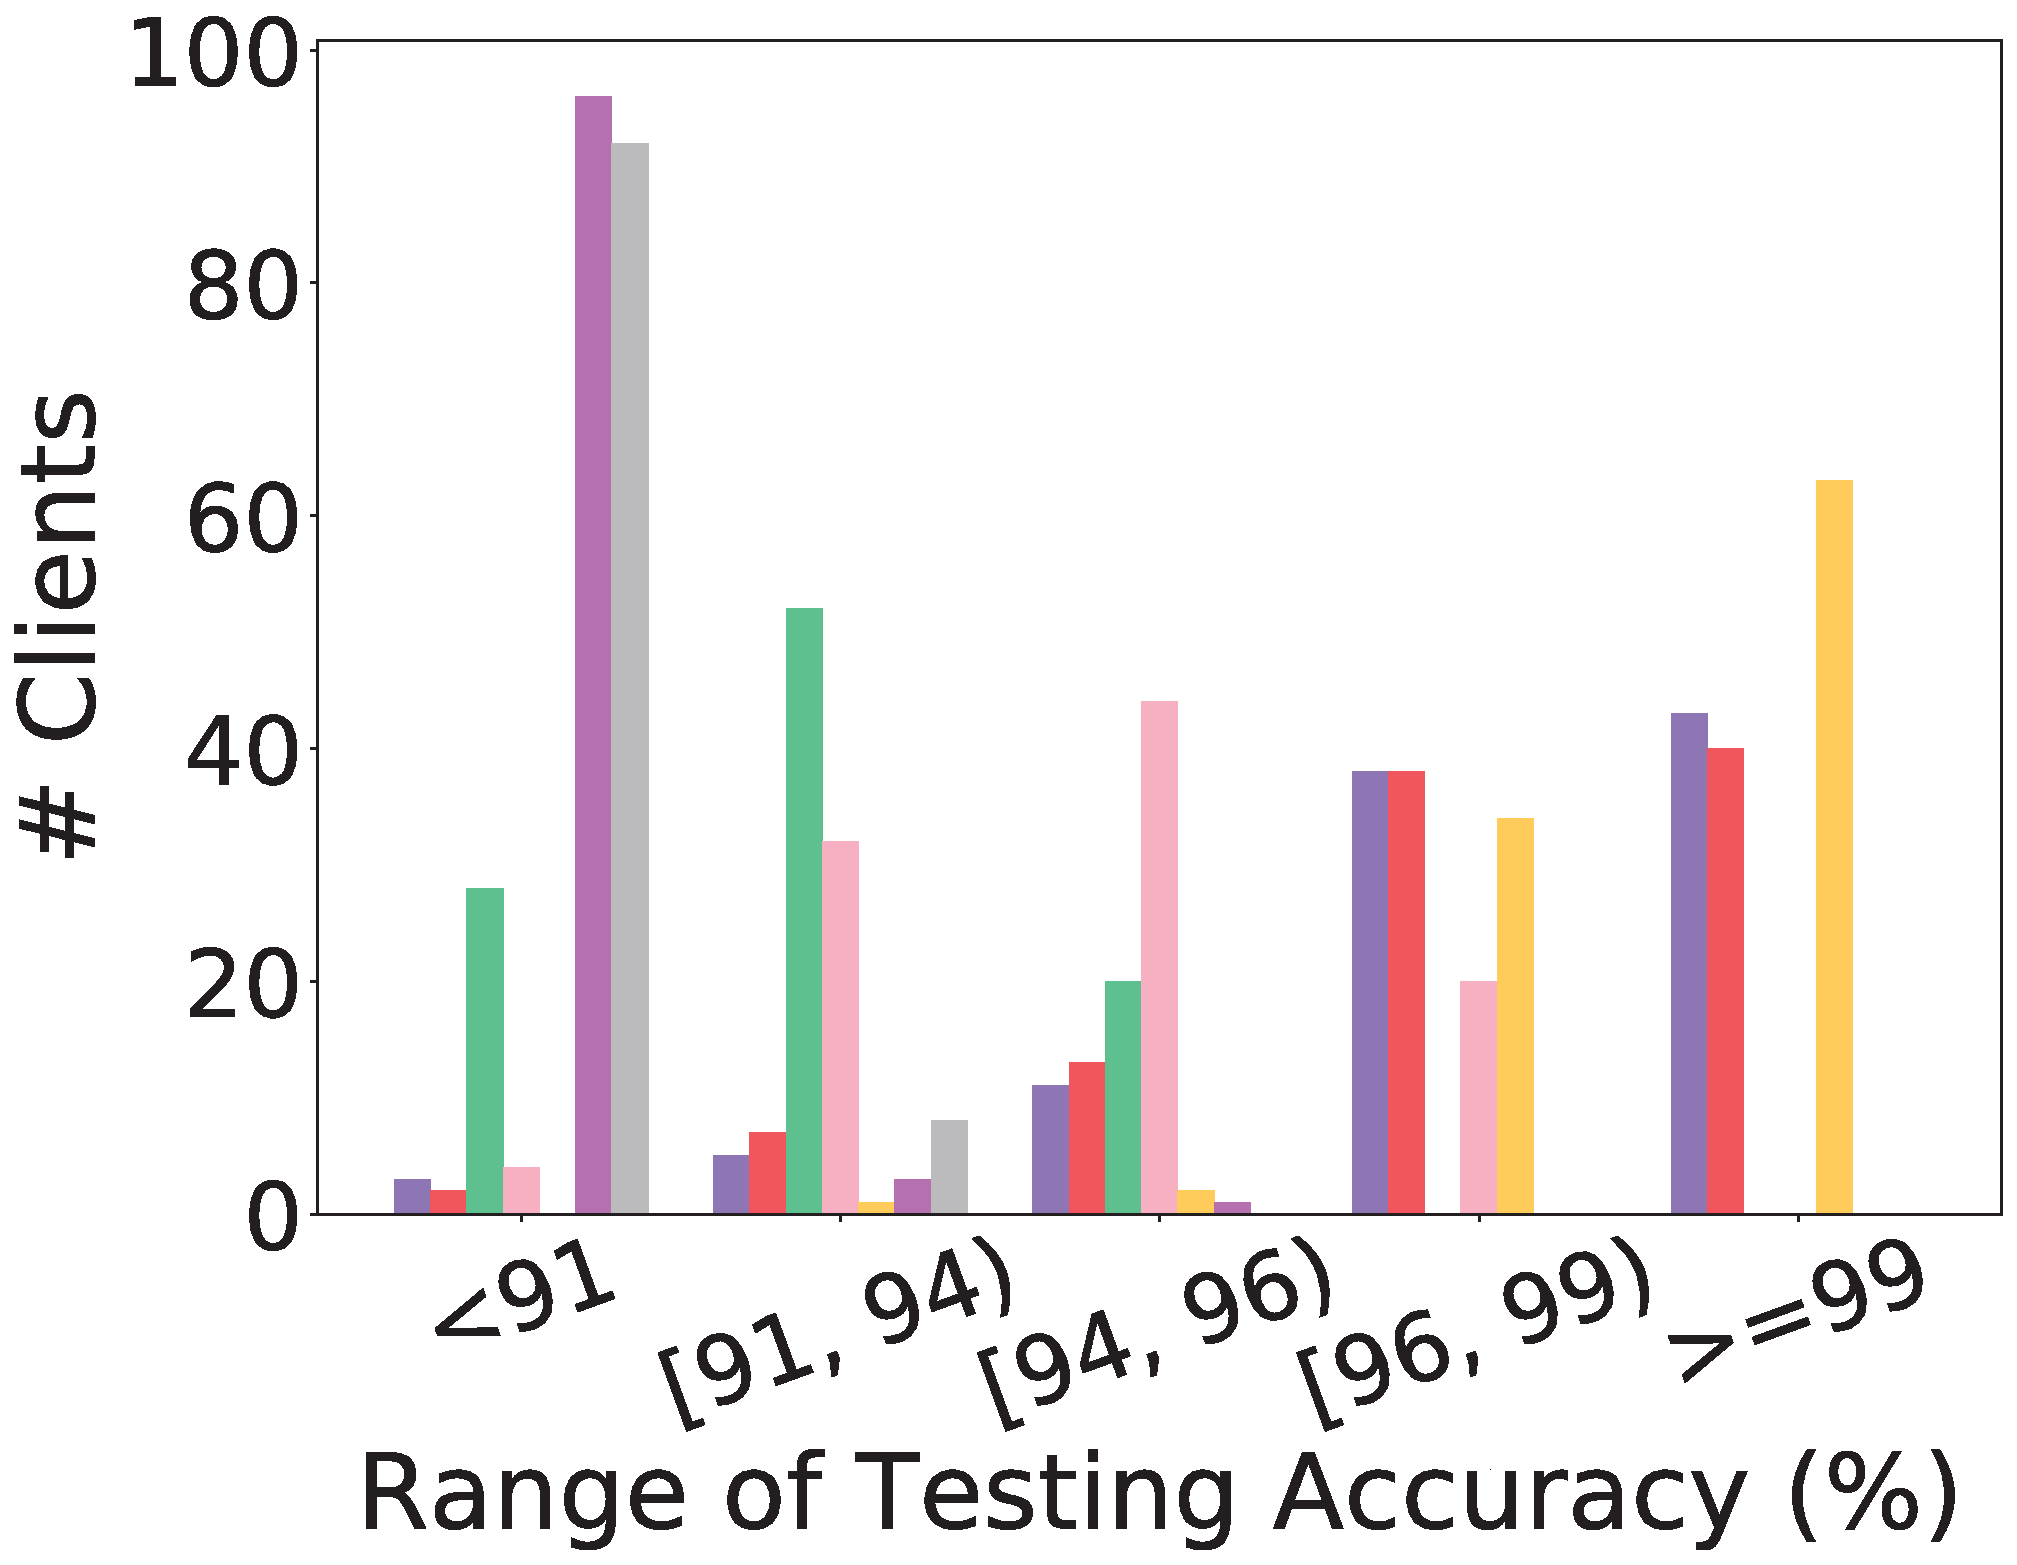
\includegraphics[width=\textwidth]{figures/Histo_MNIST_PracticalNonIID.pdf} 
        \caption{MNIST}
        \label{subfig:MNIST}
    \end{subfigure}
    \begin{subfigure}[b]{0.23\textwidth}
        \centering
        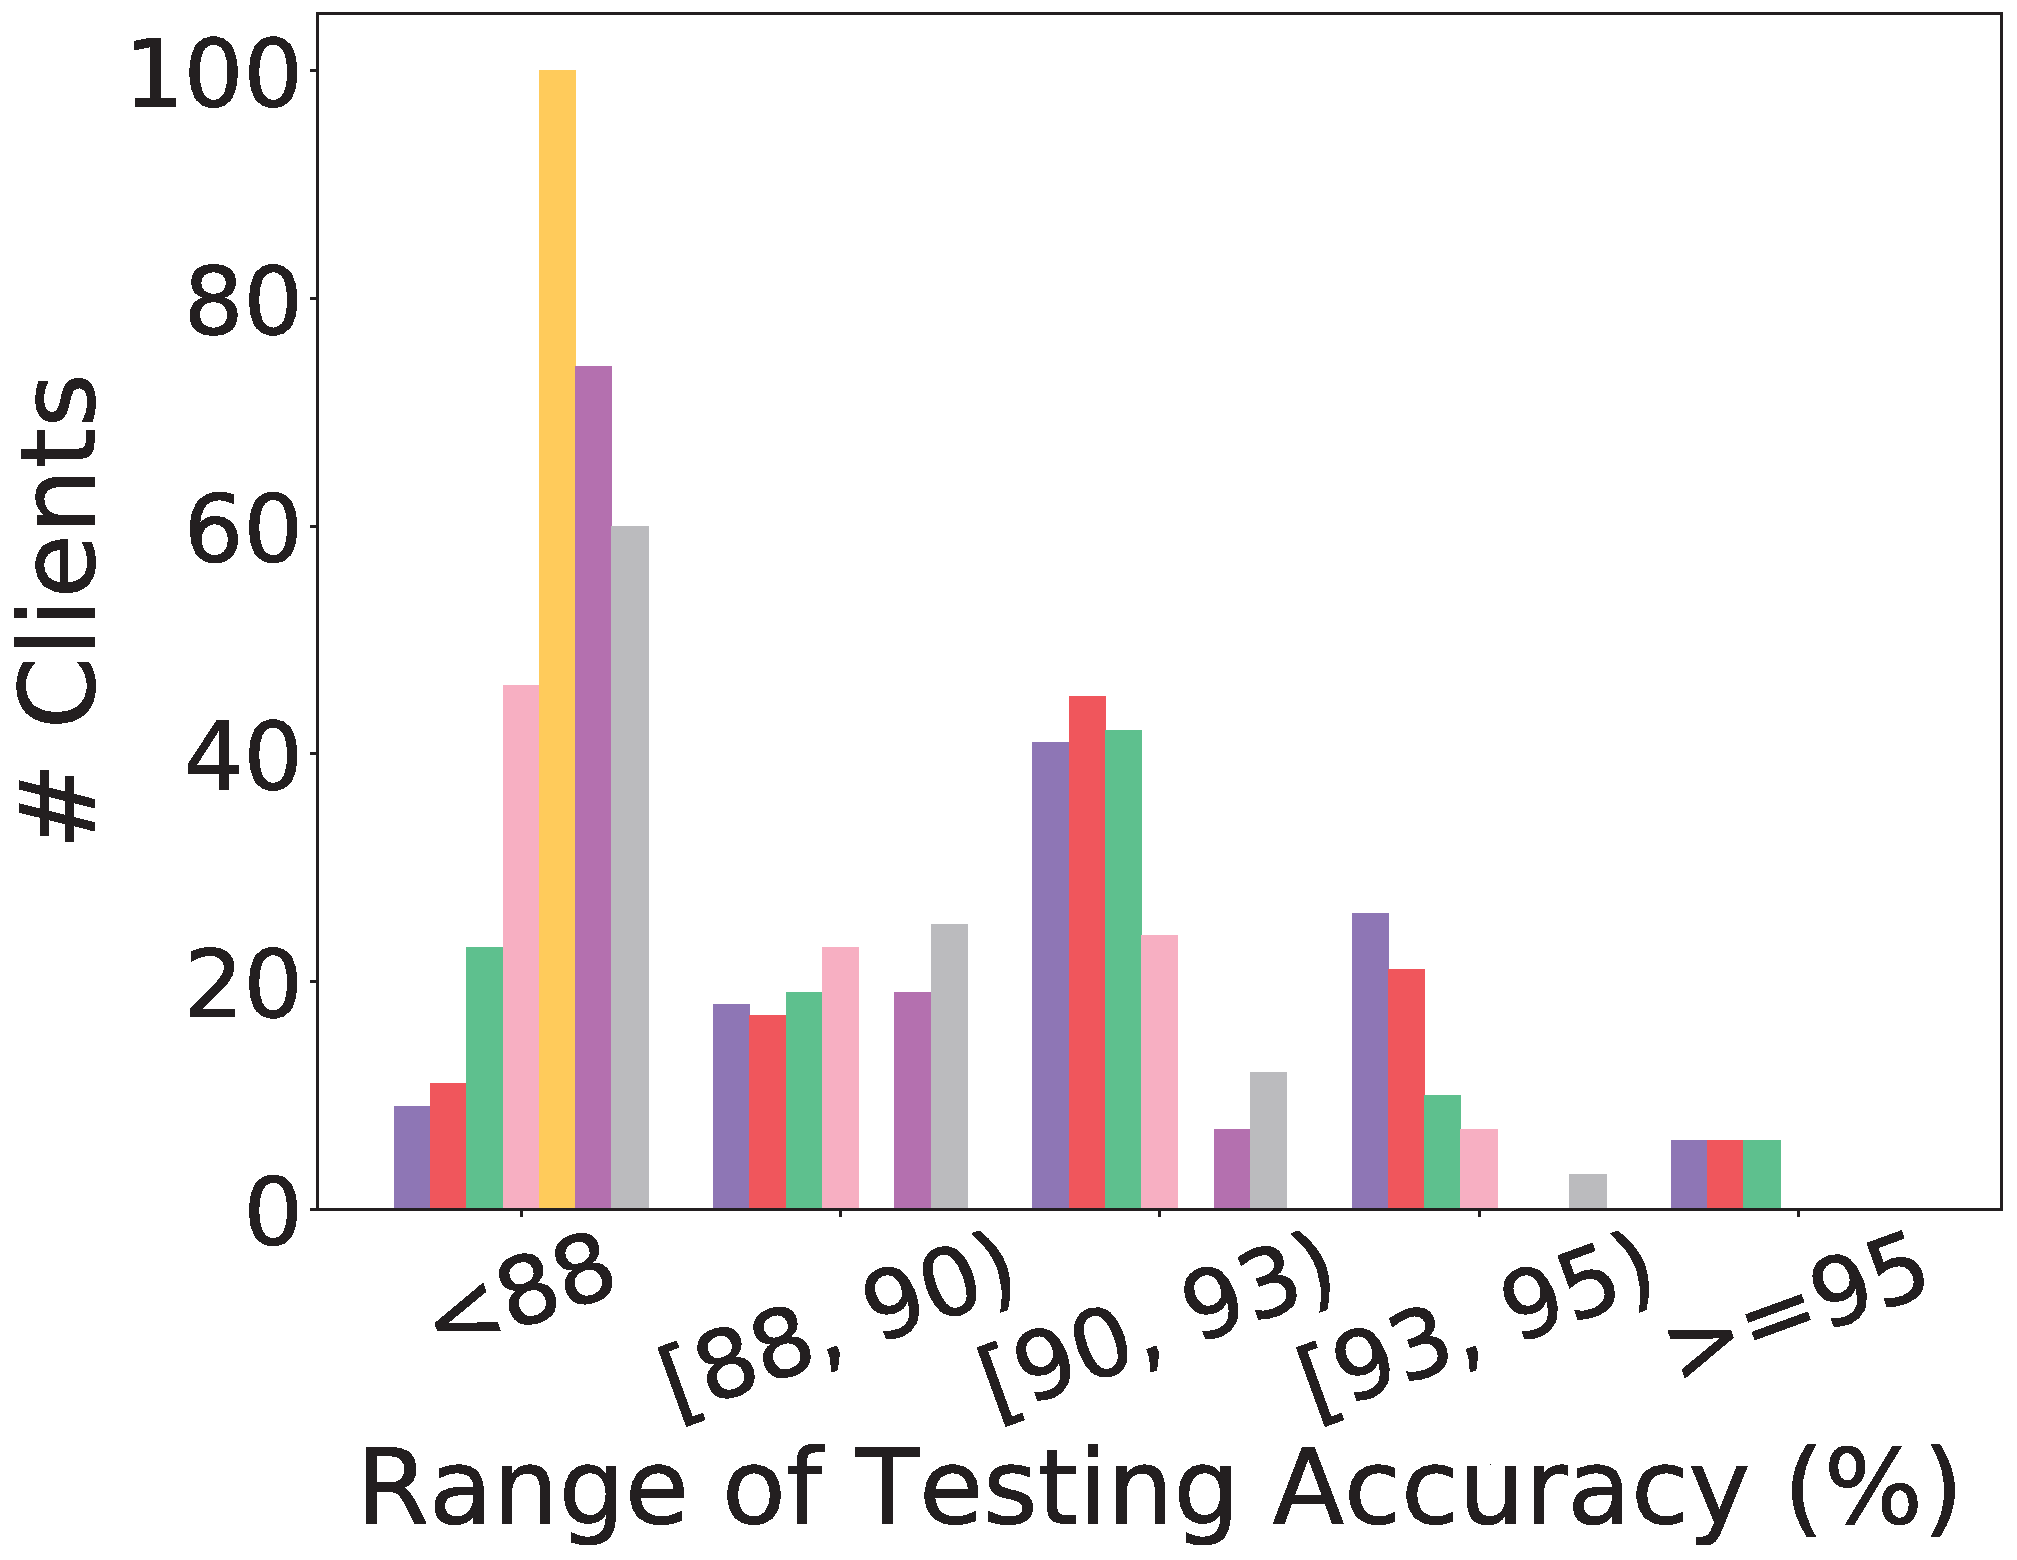
\includegraphics[width=\textwidth]{figures/Histo_FMNIST_PracticalNonIID.pdf}
        \caption{FMNIST}
        \label{subfig:FMNIST}
    \end{subfigure}
    \begin{subfigure}[b]{0.23\textwidth}
        \centering
        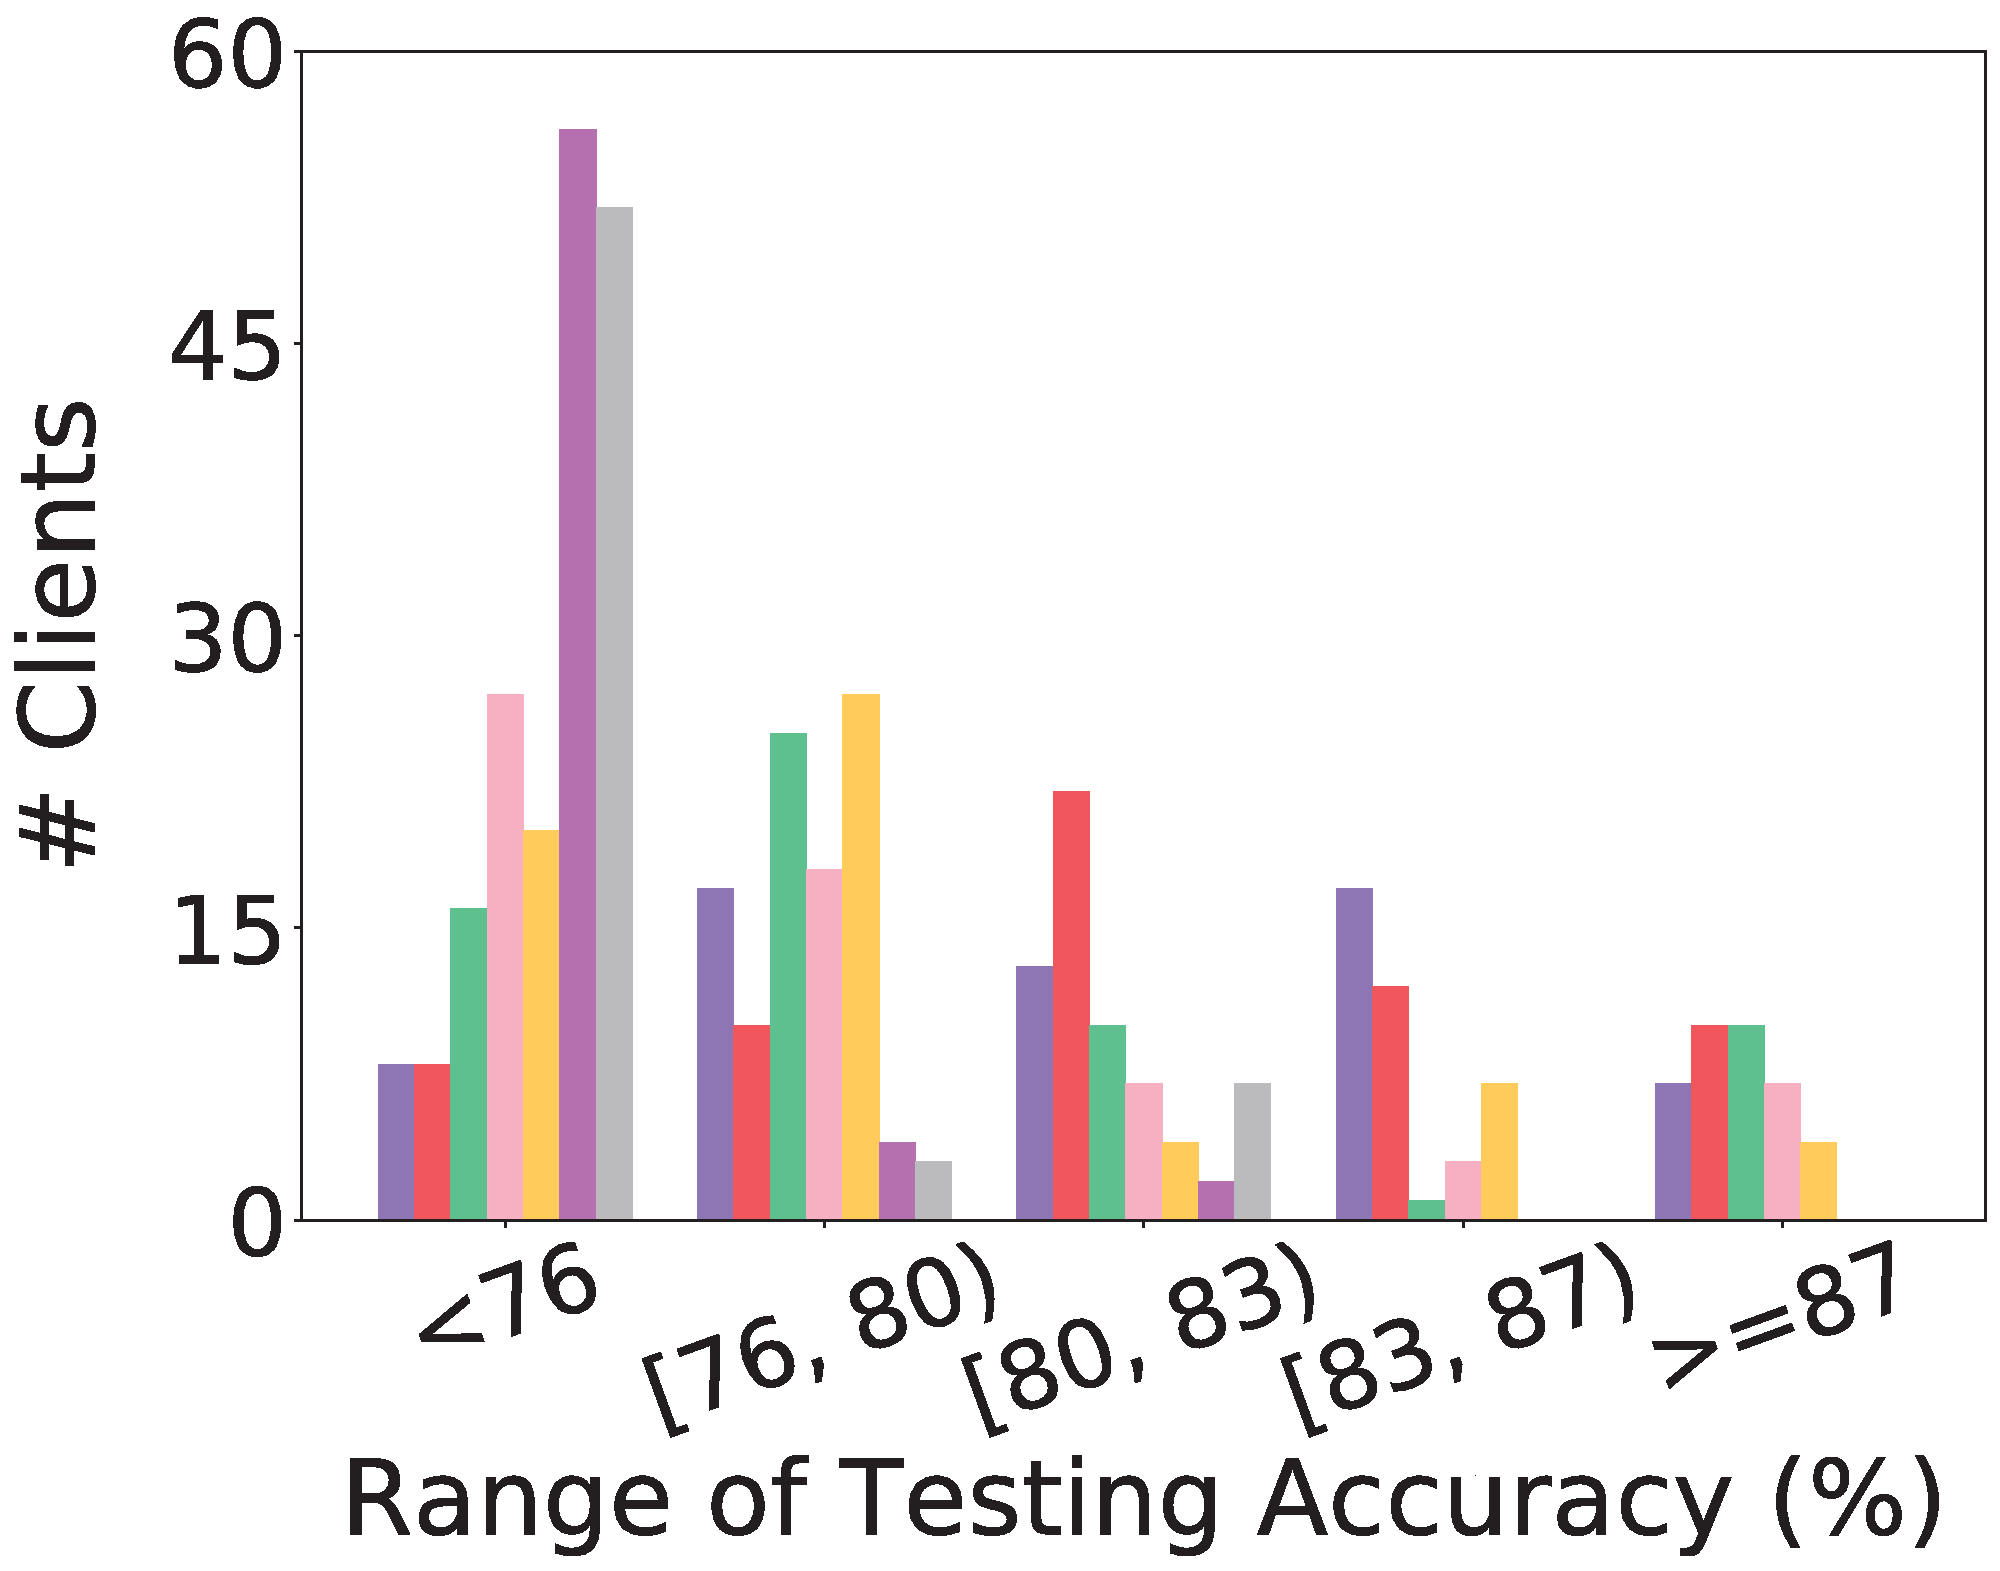
\includegraphics[width=\textwidth]{figures/Histo_EMNIST_PracticalNonIID.pdf} 
        \caption{EMNIST}
        \label{subfig:EMNIST}
    \end{subfigure}
    \begin{subfigure}[b]{0.23\textwidth}
        \centering
        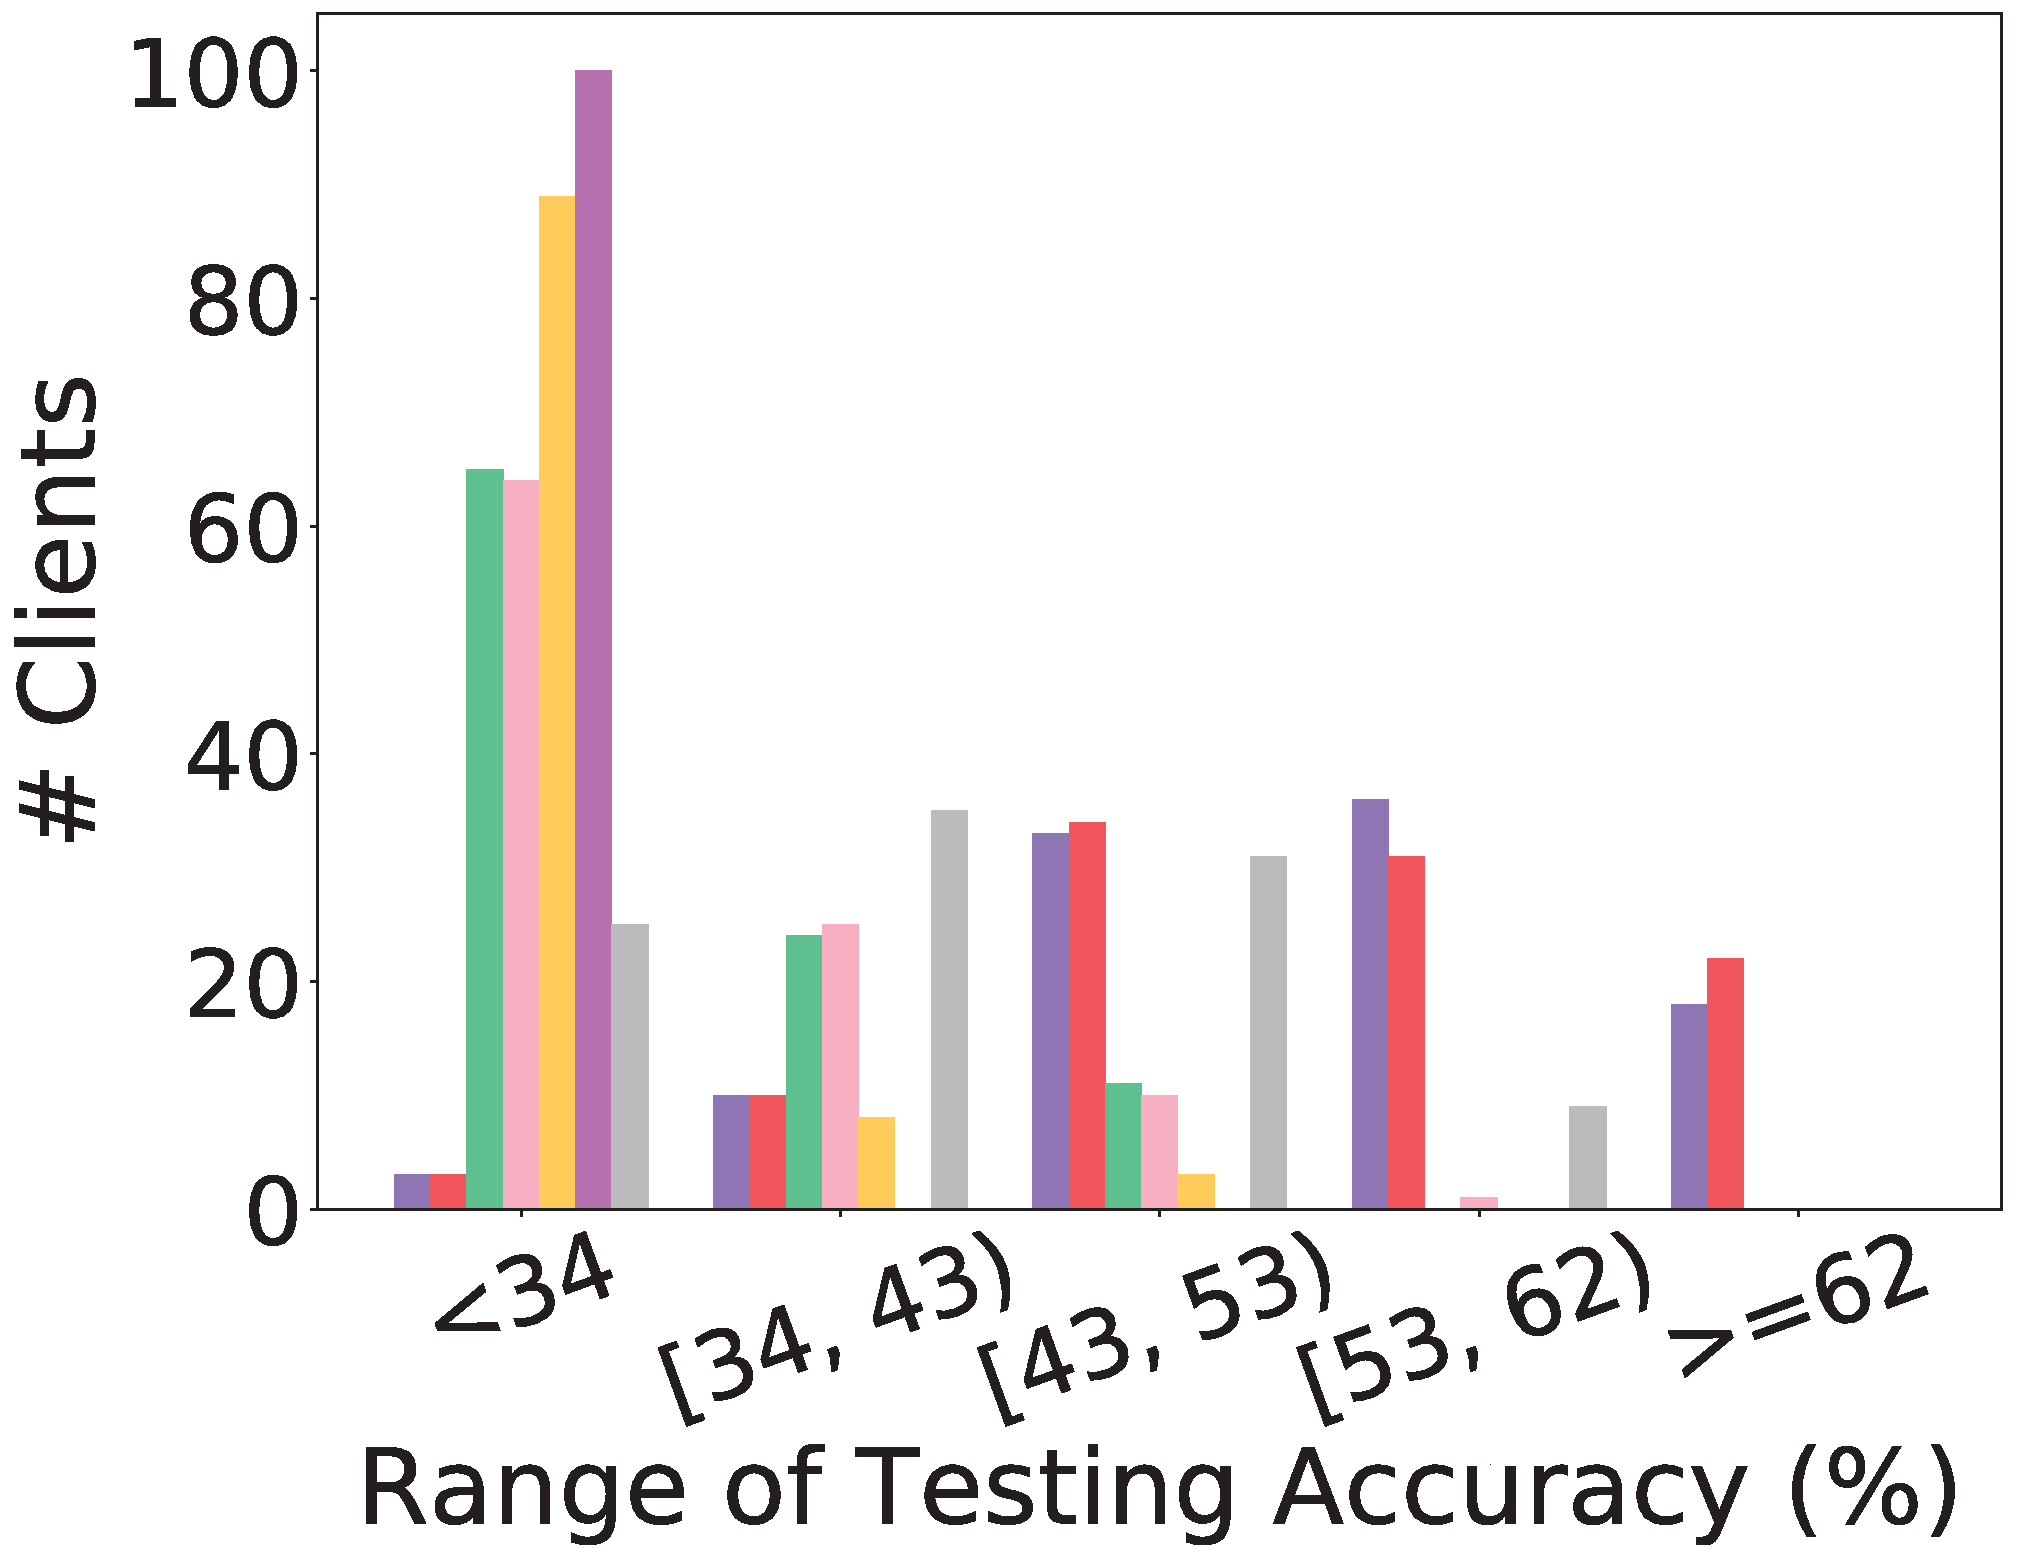
\includegraphics[width=\textwidth]{figures/Histo_CIFAR100_PracticalNonIID.pdf}
        \caption{CIFAR100}
        \label{subfig:cifar}
    \end{subfigure}
    %\caption{Histogram of the best mean testing accuracy for practical non IID.}
    \caption{The distribution of the testing accuracy of all clients under the practical non-IID data setting.}
    \label{fig:distribution}
\end{figure}

\begin{figure}[t]
    \centering
    % \begin{subfigure}[b]{0.3\textwidth}
    %     \centering
    %     \includegraphics[width=\textwidth]{figures/heatmap_fedavgprox.png}
    %     \caption{FedAvg and FedProx}
    %     \label{subfig:cluster-1}
    % \end{subfigure}
    \begin{subfigure}[b]{0.21\textwidth}
        \centering
        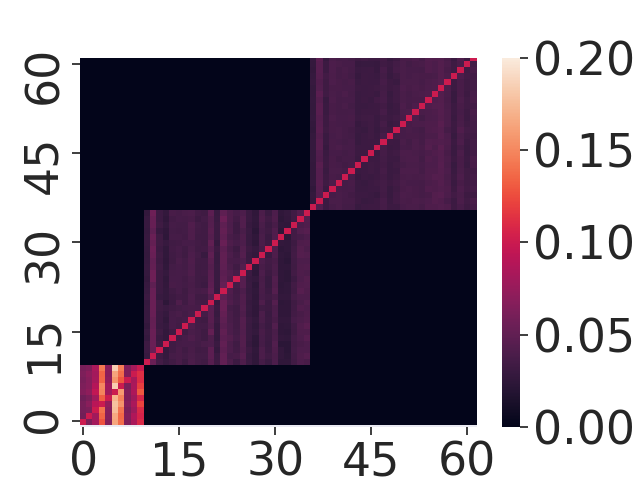
\includegraphics[width=\textwidth]{figures/heatmap_amp.png} 
        \caption{FedAMP}
        \label{subfig:cluster-1}
    \end{subfigure}
    \begin{subfigure}[b]{0.21\textwidth}
        \centering
        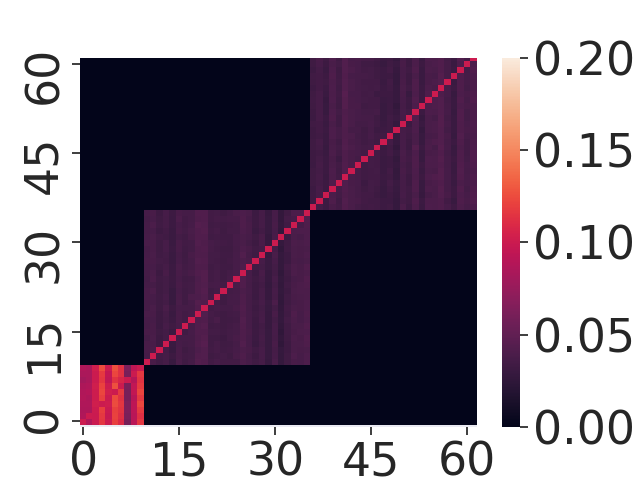
\includegraphics[width=\textwidth]{figures/heatmap_heuristic.png}
        \caption{HeurFedAMP}
        \label{subfig:cluster-2}
    \end{subfigure}
    \caption{The visualization of the collaboration weights $\xi_{i,j}$ computed by FedAMP and HeurFedAMP on EMNIST under the practical non-IID data setting. X-axis and y-axis show the IDs of clients.}
    \label{fig:cluster}
\end{figure}

% \begin{figure}
%     \centering
%     \includegraphics[width=0.4\textwidth]{figures/fedavg_histogram.png}
%     \caption{Weights for computing the global cloud model used by FedAvg/FedAvg-FT, FedProx/FedProx-FT, SCOFFLOD and APFL on EMNIST practical non-IID data set.}
%     \label{fig:weights}
% \end{figure}

% \subsection{Tolerance to Dirty Data}\label{subsec:dirtydata}
% We further explore the advantages of attentive collaboration mechanism by comparing {FedAMP} and {HeurFedAMP} with the baselines on a more practical scenario, where the training data on some clients are contaminated by dirty labels. This phenomenon is quite usual because the quality of annotations is not always good enough. To conduct this experiment, we set two out of five clients have dirty labels, and three levels are considered, where percentages of dirty labels are set as 20\%, 40\% and 60\%, respectively. We show the results of EMNIST data set in Fig.~\ref{fig:no} and more results are in the supplemental material. Fig.~\ref{fig:no} illustrates that by leveraging the attentive message passing mechanism, {FedAMP} and {HeurFedAMP} obviously outperform all other compared approaches in all levels of dirty labels in terms of the mean testing accuracy. In addition, 
% it is worthy to notice that {HeurFedAMP} is less stable as the level of dirty labels grows since there is no convergence guarantee for this heuristic method as stated in Sec.~\ref{sec:heuristic}. 

% \begin{figure}
%     \centering
%     \begin{subfigure}[b]{0.22\textwidth}
%         \centering
%         
\includegraphics[width=\textwidth]{figures/MNIST.pdf}
%         % \caption{FedAvg}
%         \label{subfig:cluster-1}
%     \end{subfigure}
%     \begin{subfigure}[b]{0.22\textwidth}
%         \centering
%         \includegraphics[width=\textwidth]{figures/FMNIST.pdf} 
%         % \caption{FedProx}
%         \label{subfig:cluster-2}
%     \end{subfigure}
%     \begin{subfigure}[b]{0.22\textwidth}
%         \centering
%         \includegraphics[width=\textwidth]{figures/EMNIST.pdf}
%         % \caption{FedProx}
%         \label{subfig:cluster-3}
%     \end{subfigure}
%     \begin{subfigure}[b]{0.22\textwidth}
%         \centering    
%         \includegraphics[width=\textwidth]{figures/cifar100.pdf}
%         \label{subfig:cluster-4}
%     \end{subfigure}
%     \begin{subfigure}[b]{0.09\textwidth}
%         \includegraphics[width=\textwidth]{figures/legend1.pdf}
%         \label{subfig:clusterlegend}
%     \end{subfigure}
    
%     \caption{Placeholder}
%     \label{fig:dirtydata}
% \end{figure}

% \begin{figure}
%     \centering
%     \begin{subfigure}[b]{0.28\textwidth}
%         \centering
%         \includegraphics[width=\textwidth]{figures/EMNIST_Noise20.pdf}
%         % \caption{$noise 20\%$}
%         % \label{subfig:no20}
%     \end{subfigure}
%         \begin{subfigure}[b]{0.28\textwidth}
%         \centering
%         \includegraphics[width=\textwidth]{figures/EMNIST_Noise40.pdf}
%         % \caption{$noise 40\%$}
%         % \label{subfig:no40}
%     \end{subfigure}
%         \begin{subfigure}[b]{0.28\textwidth}
%         \centering
%         \includegraphics[width=\textwidth]{figures/EMNIST_Noise60.pdf}
%         % \caption{$noise 60\%$}
%         % \label{subfig:no60}
%     \end{subfigure}
%         \begin{subfigure}[b]{0.14\textwidth}
%         \includegraphics[width=\textwidth]{figures/legend3.pdf}
%         % \label{subfig:nolegend}
%     \end{subfigure}
%     \caption{Performance of {FedAMP} and {HeurFedAMP} compared with baselines for different levels of dirty labels on EMNIST.}
%     \label{fig:no}
% \end{figure}

% \subsection{Tolerance to Dropped Clients}\label{subsec:dropline}
% Finally, to address the unreliable operating environment challenge in personalised federated learning, we conduct the clients dropping experiments for {FedAMP}, {HeurFedAMP} and the baselines. The results of 10\%, 30\%, and 50\% randomly dropped clients in each round for EMNIST data set are shown in Fig.~\ref{fig:dn} and those for other data sets are in the supplemental material. We clearly see that the overall mean testing accuracy of {FedAMP} and {HeurFedAMP} are better than baselines. This demonstrates  that both {FedAMP} and {HeurFedAMP} can robustly handle clients dropping.


% \begin{figure}
%     \vspace{-0.3in}
%     \centering
%     \begin{subfigure}[b]{0.28\textwidth}
%         \centering
%         \includegraphics[width=\textwidth]{figures/EMNIST_Drop10.pdf}
%         % \label{subfig:dn09}
%     \end{subfigure}
%         \begin{subfigure}[b]{0.28\textwidth}
%         \centering
%         \includegraphics[width=\textwidth]{figures/EMNIST_Drop30.pdf}
%         % \caption{$tpr=0.7$}
%         % \label{subfig:dn07}
%     \end{subfigure}
%         \begin{subfigure}[b]{0.28\textwidth}
%         \centering
%         \includegraphics[width=\textwidth]{figures/EMNIST_Drop50.pdf}
%         % \caption{$tpr=0.5$}
%         % \label{subfig:dn05}
%     \end{subfigure}
%         \begin{subfigure}[b]{0.14\textwidth}
%         \includegraphics[width=\textwidth]{figures/legend3.pdf}
%         % \label{subfig:dnlegend}
%     \end{subfigure}
%     \vspace{-0.25in}
    
%     \caption{Performance of {FedAMP} and {HeurFedAMP} compared with baselines for different ratios of dropped clients on EMNIST.}
%     \vspace{-0.2in}
%     \label{fig:dn}
% \end{figure}
